% This example is meant to be compiled with lualatex or xelatex
% The theme itself also supports pdflatex
\PassOptionsToPackage{unicode}{hyperref}
\documentclass[aspectratio=1610, 9pt]{beamer}

% Load packages you need here
\usepackage{polyglossia}
\setmainlanguage{german}

\usepackage{csquotes}


\usepackage{amsmath}
\usepackage{amssymb}
\usepackage{mathtools}

\usepackage{hyperref}
\usepackage{bookmark}

% load the theme after all packages

\usetheme[
  showtotalframes, % show total number of frames in the footline
]{tudo}

% Put settings here, like
\unimathsetup{
  math-style=ISO,
  bold-style=ISO,
  nabla=upright,
  partial=upright,
  mathrm=sym,
}

\title{Ist das Universum ein Computer?}
\author[J.~Speer]{Jannis Speer}
\date{17.12.20}
\institute{Big Questions Seminar}
\titlegraphic{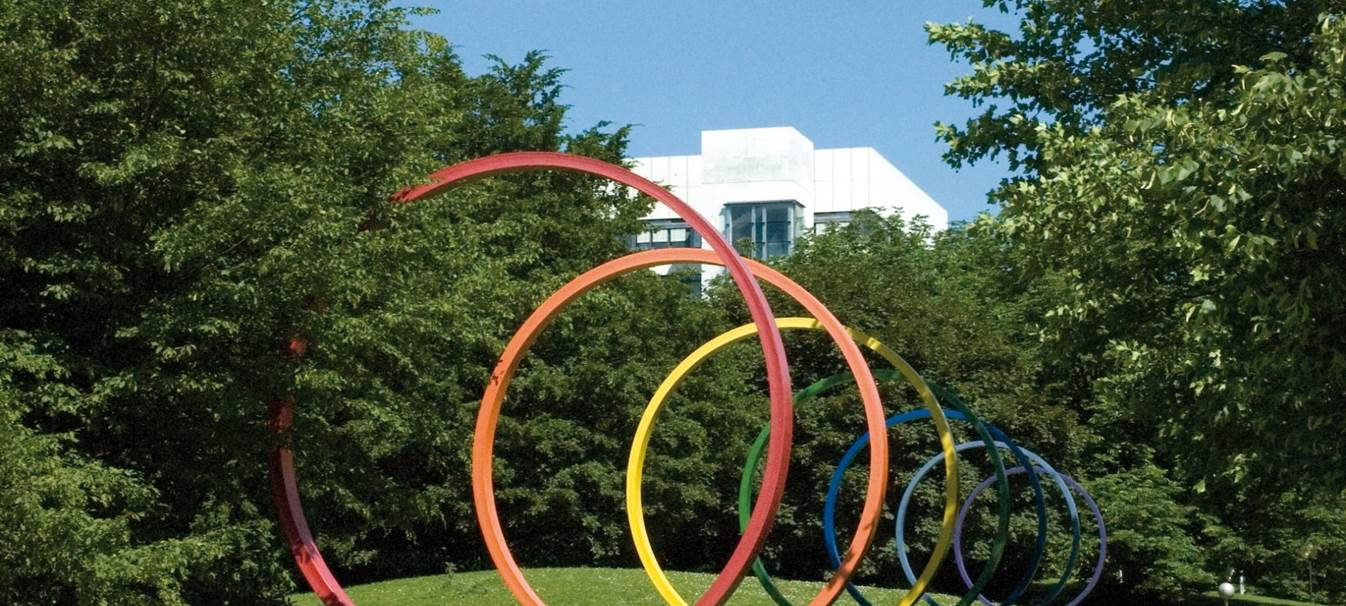
\includegraphics[width=0.7\textwidth]{images/tudo-title-2.jpg}}


\begin{document}

\maketitle

\begin{frame}{Inhalt}
  \begin{itemize}
    \item
  \end{itemize}
\end{frame}

%\begin{frame}{Inhalt}
%  \tableofcontents
%\end{frame}

\begin{frame}{Historische Einführung: Digitale Physik}
  \begin{itemize}
    \item ursprüngliche Idee: Konrad Zuses Buch Rechnender Raum (1969)
    \item Hypothese: Universum ist digitaler Computer, genauer: zellulärer Automat
    \item Komatibilität von Computern mit: \\Informationstheorie, statistischer Mechanik, Quantenmechanik
    \item Begriff geprägt durch  Edward Fredkin, alternativ: digitale Philosophie
    \item[]
    \item[\rightarrow] Digitale Physik: Theorien mit Prämise, Universum durch Information beschreibbar ist
  \end{itemize}
\end{frame}

\begin{frame}{Digitale Physik - verschiedene Perspektiven}
  \begin{itemize}
    \item Weizsäckers Quantentheorie der Ur-Alternativen:
      \begin{itemize}
        \item[\bullet] lediglich 2  Entitäten: Struktur der Zeit, binäre Alternativen
        \item[\bullet] abstrakt, nicht-lokal, keine feldtheoretischen Voraussetzungen
      \end{itemize}
    \item[]
    \item Wheelers It from Bit:
      \begin{itemize}
        \item[\bullet] klassisch: Realität existiert und wird gemessen
        \item[\bullet] hier: Messung schafft Realität
      \end{itemize}
    \item[]
    \item Pancomputationalism:
      \begin{itemize}
        \item[\bullet] Digitaler Computer vs. Quantencomputer
        \item[\bullet] Zufälligkeit und Komplexität des Universums? Effizienz?
      \end{itemize}
    \item[]
    \item Tegmarks Mathematical-Universe-Hypothese (MUH)
      \begin{itemize}
        \item[\bullet] Universum ist Mathematik, mathematische Existenz = physikalische Existenz
      \end{itemize}
  \end{itemize}
\end{frame}

\begin{frame}{Informationstheorie}

\end{frame}

\begin{frame}{Algorithmische Informationstheorie}

\end{frame}

\begin{frame}{Digitale Information, Boolesche Algebra, Klassische Logik}

\end{frame}

\begin{frame}{Vor Turing}

\end{frame}

\begin{frame}{Turingmaschine}

\end{frame}

\begin{frame}{Turingmaschine 2}

\end{frame}

\begin{frame}{Implementierung einer Turingmaschine}

\end{frame}

\begin{frame}{Universum als digitaler Computer}

\end{frame}

\begin{frame}{Universum als digitaler Computer 2}

\end{frame}

\begin{frame}{Effizienz von digitalen Computern}

\end{frame}

\begin{frame}{Quantencomputer}

\end{frame}

\begin{frame}{Quantencomputer 2}

\end{frame}

\begin{frame}{Universum als Quantencomputer}

\end{frame}

\begin{frame}{Universum als Quantencomputer 2}

\end{frame}

\begin{frame}{Digitaler Computer vs. Quantencomputer}

\end{frame}

\begin{frame}{Das Universum ist kein Computer}

\end{frame}

\begin{frame}{Ausblick}

\end{frame}

\end{document}
